\documentclass[12pt]{article}
\usepackage{graphicx}
\usepackage{caption}
\usepackage{subfig}
\usepackage{geometry}
\usepackage{amsfonts}
\usepackage{amsmath}
\usepackage{amsthm}
\usepackage{xcolor}
\usepackage{setspace}

\newcommand{\abs}[1]{\lvert #1 \rvert}
\usepackage{indentfirst}
\newtheorem{lemma}{Lemma}[section]
\geometry{letterpaper, portrait, margin=1in}
\setlength{\parindent}{0cm}
\numberwithin{equation}{section}
\numberwithin{figure}{section}
\begin{document}


\onehalfspacing
\setlength\parindent{24pt}

\begin{center}


625.721 Final Project: Simulation of Wind Direction over the Atlantic Ocean

\null

Matthew LeDuc


\end{center}
\section{Introduction}

The theory of statistics on convex subsets of $\mathbb{R}^n$ has been studied since at least the 7th century, when the Arab scholar Al-Khalil used permutations and combinations to list all possible Arabic words with and without vowels \cite{Broemling}. However, there are several areas relevant to daily life when the methods of linear statistics break down completely. For example, we know that the time halfway between 23:00 and 01:00 hours is 00:00 hours, however taking the average of 23 and 1 leads us to believe that the halfway time is 12:00 hours. We also know that the compass direction between 315 degrees (NW) and 45 degrees (NE) is not 180 degrees (S) but actually 0 deg (N), a difference of 180 degrees! Setting your compass this way would leave you hopelessly lost (ask me how I know). For this reason, over the last century the field of directional or circular statistics has been growing incredibly rapidly, starting with Richard von Mises studying the deviation of atomic weights from integer values and continuing into the present day \cite{Mardia2}.  At present, the field finds applications in modeling of temporal variations in environmental phenomena such as wind and wave direction, in the modeling of the migration patterns of birds, protein folding, and in any other area that can be assumed to be taking place on $\mathbb{S}^n$, the $n-$cylinder, or the $n-$torus. Many great examples of these sorts of processes can be found in the references, in particular in \cite{Craig}, \cite{Kanti}, and \cite{Mardia2}. 

Many papers have focused on the modeling of distributions of wind direction (see \cite{Al Yammahi}, \cite{Craig}, and \cite{Mahrt}, among many others, for examples). This is of particular interest to many people in industry and government, who want to know how such variations might affect, for example, the output of a wind power plant. We will continue to follow this trend in this paper. We will investigate the use of these techniques on data from the National Data Buoy Center to model time series of wind direction measured over the Atlantic Ocean.

\section{Circular Statistics}

Circular data can be represented as angles or as complex numbers on the unit circle. This means that a given datapoint can be represented in multiple ways, such as as an angle $\theta$, as a unit vector $(\cos \theta, \sin \theta)^T$, or as a complex number $e^{i\theta}$. Each of these representations is useful for different applications and each will be used in this work. In addition, there are multiple ways to represent the values of the angles themselves and multiple ways to select the $0$ point and positive direction of rotation. However, in spite of these possibilities we want two people who are obsesrving the same data but using different conventions to be able to get the same results. This invariance to coordinates is the main issue that separates ordinary statistics, where it is almost never worried about, and circular statistics. In this section we will discuss the definitions of common statistical quantities on the circle, which will allow us to analyze data and do comparisons in a similar way to ordinary statistics.

\subsection{The Mean}\label{mean}

Consider a set of unit vectors $x_1, ..., x_n$ with corresponding angles $\theta_1, ..., \theta_n$. One intuitive way to find the mean is by setting $z_k = e^{i \theta_k}$, in which case $\bar{z} = \frac{1}{n}\sum_{k=1}^n z_k$. Then the \textit{mean resultant length} $R = \|\bar{z}\|$ and the \textit{mean direction} is given by $\bar{\theta} = \angle \bar{z}$. The mean $\bar{z}$ represents the location of the center of mass of the datapoints. If we chose not to convert to complex numbers, we could find the angular mean by bearing in mind its relationship with the center of mass of the datapoints. The mean direction is the direction of the sum $x_1+...+x_n$. Since the coordinates of each $x_k$ are given by $(\cos \theta_k, \sin \theta_k)^T$, the coordinates of the center of mass of the datapoints $(\bar{C}, \bar{S})^T$ are given by 

\begin{equation}\label{eq:CandS}
\begin{aligned}
\bar{C} = \frac{1}{n}\sum_{k=1}^n \cos \theta_k \\
\bar{S} = \frac{1}{n}\sum_{k=1}^n \sin \theta_k \\
\end{aligned}
\end{equation}
and $R$ and $\bar{\theta}$ are the solutions to the system of equations

\begin{equation}\label{eq:RandT}
\begin{aligned}
\bar{C} = R \cos \bar{\theta} \\
\bar{S} = R \sin \bar{\theta}
\end{aligned}
\end{equation}
assuming $R>0$. Then the value of $R$ can be assumed from trigonometry to be $R = \sqrt{\bar{C}^2+\bar{S}^2}$, and the value of $\bar{\theta}$ can be found using the four-quadrant arctangent function \cite{Kanti}. The mean resultant length $R$ is between $0$ and $1$, being close to $0$ when the data is spread over the circle and close to $1$ when it is highly concentrated. Thus, it can be thought of as a measure of the concentration of a dataset. However, we should note that the data set made by $\theta_1, ..., \theta_n, \theta_1+\pi, ..., \theta_n+\pi$ has $R=0$, so $R=0$ does not imply that the data is spread evenly over the circle, only that the datapoints are spread symmetrically.

\subsection{Variance, Dispersion, and Standard Deviation}

For most applications, $R$ is perfectly adequate as a measure of spread \cite{Kanti}, however it is sometimes necessary to consider other measures for comparison with ordinary data. The \textit{circular variance} is defined as

\begin{equation}\label{eq:circvar}
V = 1-R
\end{equation}
and since $0\le R\le 1$, it follows that $0 \le V \le 1$ as well.

We may also wish to consider the dispersion of a set of angles. We do this by considering a useful measure of angular distance: the cosine distance given by 

\begin{equation}\label{eq:cosdist}
\delta = 1-\cos(\theta_1-\theta_2)
\end{equation}

This naturally suggests one way of measuring dispersion of a set of angles about a given angle $\alpha$:

\begin{equation}\label{eq:disp}
D(\alpha) = \frac{1}{n}\sum_{k=1}^n (1-\cos(\theta_k-\alpha))
\end{equation}

It can be shown that equation \ref{eq:disp} has a minimum of $V$ at $\alpha = \bar{\theta}$, which is analogous to the result on the line that $\frac{1}{n}\sum_{k=1}^n(x_k-u)^2$ takes on a minimum at $u=\bar{x}$, and that value is a biased estimator of the sample variance \cite{Kanti}. 

We can derive an analogue for the standard deviation by transforming the variance $V$. One appropriate statistic is the sample \textit{circular standard deviation} given by

\begin{equation}\label{eq:stdev}
v = \sqrt{-2 \log(1-V)} = \sqrt{-2 \log(R)}
\end{equation}
which takes values on $\mathbb{R}_{\ge 0}$ instead of $[0,1]$. For small values of $V$ this takes the form

\begin{equation}\label{eq:smallstdev}
v \approx \sqrt{2(1-R)}
\end{equation}
The easy analogue to ordinary statistics leads some authors to refer to $2(1-R)$ as the circular variance instead of equation \ref{eq:circvar} \cite{Kanti}.

\subsection{Trigonometric moments}

Recall from equation \ref{eq:CandS} that $\bar{C}$ and $\bar{S}$ are defined as the average cos/sin respectively of the angles $\theta_k$. As alluded to in section \ref{mean}, these are related to the mean resultant length and the mean direction of the $x_k$. They can be combined to form the \textit{first trigonometric mement about zero} given by

\begin{equation}\label{eq:1sttm}
m'_1 = \bar{C}+i\bar{S} = R e^{i\bar{\theta}}
\end{equation}

This can be extended to define the \textit{$p^{th}$ trigonometric moment about zero} for $p=1,2,3,...$ by writing

\begin{equation}\label{eq:pthtm}
\begin{aligned}
m'_p = a_p+ ib_p\\
a_p = \frac{1}{n}\sum_{k=1}^n \cos(p\theta_k)\\
b_p = \frac{1}{n}\sum_{k=1}^n \sin(p\theta_k)\\
\end{aligned}
\end{equation}

Then, one can see from euler's formula that $m_p = R_pe^{i\bar{\theta_p}}$, where $R_p$ and $\bar{\theta_p}$ are the mean resultant length and direction of the data $p\theta_1, ..., p\theta_n$. The $p^{th}$ moment about the mean $m_p$ is calculated in the same way, however the argument of the trigonometric function is $p(\theta_k-\bar{\theta})$ instead. It can be shown that $m_1 = R$. The population moments will be introduced in our discussion of distributions on the circle.

Now that we have a handle on common summary statistics on the circle, we can move to a discussion of common distribution functions on the circle, and then to models for data on the circle. 

\section{Distributions on the Circle}

Now that we have seen the basics of circular statistics, we will introduce the most important circular probability distributions. 

\subsection{The circular uniform distribution}

The easiest generalization from the real line to the circle is the uniform distribution. This is given by the probability density

\begin{equation}\label{uniformpdf}
f_X(x) = \frac{1}{2\pi} 
\end{equation}
which has the associated distribution function 

\begin{equation}\label{uniformcdf}
F_X(x) = \frac{x}{2\pi}
\end{equation}

This has all the same properties as the uniform distribution of the real line, so we will not spend time discussing it in detail. 

\subsection{The von Mises Distribution}
There are several different distributions that can be used for modeling wind direction data, however the most common is the von Mises distribution \cite{Al Yammahi}. Its probability density function is given by

\begin{equation}\label{eq:vm}
f_{X}(x) = \frac{e^{\kappa \cos(x - \mu)}}{2\pi I_0(\kappa)}
\end{equation}
and its cumulative density function is given by \cite{Kanti}

\begin{equation}\label{eq:vmcdf}
F_X(x) = \frac{1}{I_0(\kappa)}\int_0^x e^{\kappa \cos(x-\mu)}dx
\end{equation}

where $\mu$ is the angular mean, $\kappa \in [0,\infty)$ is a parameter that determines the spread of the distribtuion, and $I_0(\kappa)$ is the zeroth order modified Bessel function of the first kind given by 

\begin{equation}\label{eq:I0}
I_r(\kappa) = \frac{1}{2\pi} \int_0^{2\pi}\cos( r \theta )e^{\kappa\cos(\theta )} d\theta, r = 0,\pm 1, \pm 2,...
\end{equation}

We will denote the von Mises distribution with parameters $\mu$ and $\kappa$ by $M(\mu, \kappa)$. The population mean direction is given by $\mu$, and the asymptotic expanaion for the mean resultant length is given by 

\begin{equation}\label{eq:smallkappa}
R = \frac{\kappa}{2}\{ 1-\frac{1}{8}\kappa^2+\frac{1}{48}\kappa^4-\frac{11}{3072}\kappa^6+... \}
\end{equation}
for small values of $\kappa$ and 

\begin{equation}\label{eq:largekappa}
R = 1-\frac{1}{2\kappa}-\frac{1}{8\kappa^2}-\frac{1}{8\kappa^3}+o(\kappa^{-3})
\end{equation}
for large values of $\kappa$ \cite{Kanti}.
\subsubsection{Maximum Likelihood Estimation}

We will determine the approximate distribution of the wind direction via maximum likelihood estimation. Consider a set of $n$ data points $ x_1, x_1, ...,x_n $that are drawn from some distribution $f_X(x;\theta)$ where $\theta$ is an unknown parameter or vector of parameters. We can estimate $\theta$ by means of maximizing the likelihood function of the distribution. The likelihood function for $\theta$ is given by

\begin{equation}\label{eq:likelihood fn}
L(\theta) = \prod_{k=1}^n f_X(x_k|\theta)
\end{equation}

and the maximum likelihood estimate is the value $\hat{\theta}$ such that $L(\hat{\theta}) \ge L(\theta)$ for all values of $\theta$ and is the solution of the equation $\nabla L(\theta) = 0$, or equivalently $\nabla \log(L(\theta)) = 0$ (called the log-likelihood) which can often reduce the difficulty of the computation \cite{Larsen}. The log-likelihood function for the von Mises distribution given $n$ data points is given by 

\begin{equation}\label{eq:vmll}
\log(L(\kappa, \mu)) = -n\log( 2\pi I_0(\kappa))+ \sum_{k=1}^n e^{\kappa \cos(x_k-\mu)}
\end{equation}

Taking the appropriate gradient and setting it to zero, we can derive the maximum likelihood estimators $\hat{\mu}$ and $\hat{\kappa}$. Let the data points $x_1, x_2, ..., x_n$ be drawn from the interval $[0,2\pi)$ according to some distribution and consider the transformation $z_k = e^{i x_k}$. Then the smaple mean is given by $\bar{z} =\frac{1}{n}\sum_{k=1}^n z_k$ and the maximum likelihood estimate for $\mu$ is given by $\hat{\mu} = \angle\bar{z}$. The estimator for $\kappa$ is given by \cite{borradaile}

\begin{equation}
\label{eq:kmle}
\bar{R} = \frac{I_1(\hat{\kappa})}{I_0(\hat{\kappa})}
\end{equation}

where $\bar{R} = \|\bar{z}\|$. This equation can be solved via your favorite rootfinding algorithm. The author's favorite rootfinding method is the Newton-Rhapson algorithm so it is employed in this paper. As a side note, this expression combined with the power series expansions for $I_1(\kappa)$ and $I_0(\kappa)$ are how the expressions in equations \ref{eq:smallkappa} and \ref{eq:largekappa} are derived. 

%\subsection{The Kuiper Test}
%
%In ordinary statistics, it is common to use the Kolmogorov-Smirnov test to determine equality of two distributions by comparing the maximum difference between their cumulative distribution functions to a test statistic. 


\section{NDBC Data}

Our dataset of interest is the NOAA National Data Buoy Center wind direction data \cite{NDBC}. The NDBC operates a network of buoys and coastal stations throughout the world that provide important oceanograhic and atmospheric data such as wind speed and direction, significant wave height, sea surface temperature, and barometric pressure. These observations are used by federal, state, academic, and private stakeholders for weather forecasting, developing oceanic and atmospheric models, environmental monitoring, and many other purposes \cite{NDBCdoc}. For the purposes of this work, we will focus on data from buoys 41010 and 41047 collected in 2019 and 2020. The buoys are both in the Atlantic Ocean near the United States, with buoy 41010 on the Blake Plateau and buoy 41047 near the Hatteras Plain (see figure \ref{fig:buoys}). 

\begin{figure}[h]
\centering
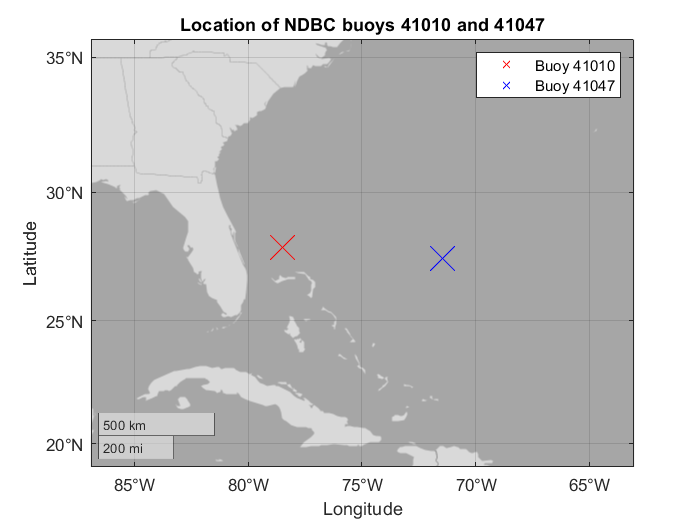
\includegraphics[width=80mm]{New Folder/buoy locations.png}
\caption{Location of NDBC buoys 41010 (red) and 41047 (blue)}\label{fig:buoys}
\end{figure}

The buoy anemometers are approximately 4 m above sea level, and wind direction data is reported every 10 minutes as integer angles in the interval $[0,360)$ measured clockwise from north. The data for each year is written into a text file, with each line representing one 10 minute time period (shown in figure \ref{fig:41047}, wind direction data is in the column titled WDIR). For our purposes, we will split the data up by month in an attempt to minimize seasonal affects. Missing values are represented by values of either 99.0 or 999.0 depending on the data column, which makes them easy to filter out. When there are only a few isolated missing data points, they are replaced by taking the angular average of the data points on either side. If they are not isolated, the month of data is not processed. This is not usually an issue that we come across in this dataset. Once the data has been read in, it is converted from angles in $[0,360)$ to $[-\pi,\pi)$ for processing. This data is matched to a von Mises distribution by means of maximum likelihood estimation for the purposes of modeling. 

\begin{figure}[h]
\centering
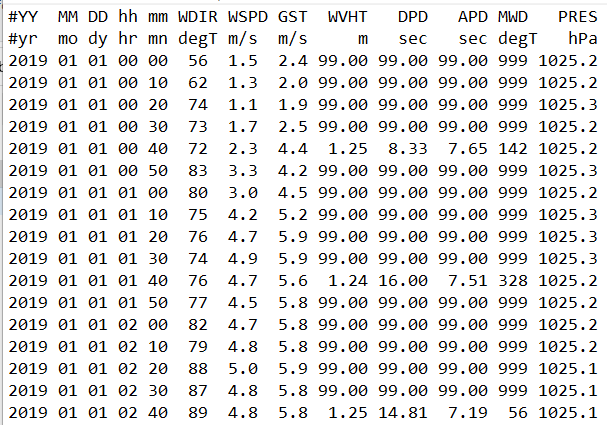
\includegraphics[width=80mm]{New Folder/ndbc screeenshot.png}
\caption{Screenshot of raw data for NDBC buoy 41047}
\label{fig:41047}
\end{figure}


\section{Modeling}

Over the years, a variety of models have been introduced for generating data with a proper directional distribution. In this section, we will explore two common ways of generating circular data: The binding density method for generating Markov processes on the circle and the von Mises process, which is a circular analogue of the Ornstein-Uhlenbeck process. We will first discuss autocorrelation and its definition for circular data, as in order ot generate realistic data we need to be able to generate data with a substantial autocorrelation. 

\subsection{Correlation of circular data}\label{correlation}

The autocorrelation of a stochastic process is the Pearson correlation of values of the process separated by a given length of time. If the process $\{X_t\}$ has zero mean and time independent variance, then the autocorrelation function is given by

\begin{equation}\label{eq:autocorr}
\rho_{X}(\tau) = E\left[X_t \bar{X}_{t+\tau}\right]
\end{equation}
where $\bar{X}$ denotes the complex conjugate. Because of the fact that the mean and variance are time independent, the autocorrelation only depends on the distance betrween samples and therefore $\rho_{X}(\tau)$ is an even function of the lag $\tau$  \cite{Gubner}. It also achieves a maximum value of $E\left[X_t^2\right]= \textnormal{Var}(X_t)$ for zero-mean processes. However, this definition of the autocorrelation is used for data drawn from the real line, and our data is drawn from the unit circle. Therefore, this definition of the autocorrelation may not be appropriate for use in our situation.

As we can readily see from any selection of data (such as what is presented in figure \ref{fig:ex ac}), real wind direction data is highly autocorrelated. There are several competing definitions of the sample autocorrelation, however we will follow the definition of the sample correlogram used in \cite{fisher}. This will allow us to select an appropriate model and parameters for our data generation by means of matching the sample correlogram.

\begin{figure}[h]
\centering
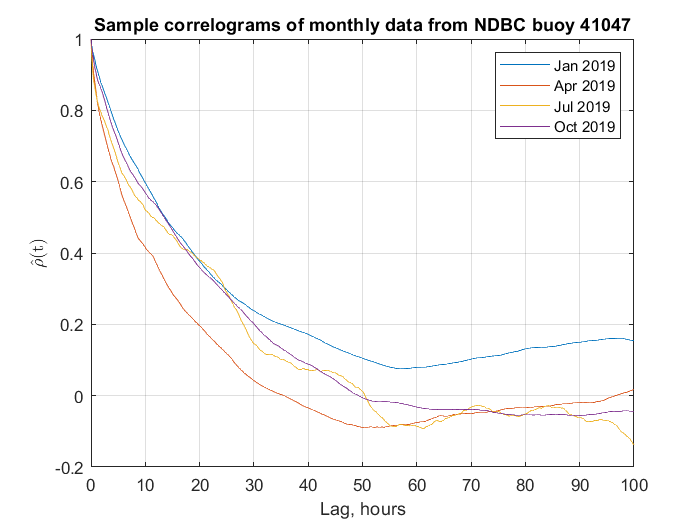
\includegraphics[width=85mm]{New Folder/example correlograms.png}
\caption{Autocorrelation of NDBC buoy data from buoy 41047}\label{fig:ex ac}
\end{figure}

The sample correlogram $\hat{\rho}(\tau)$ as defined in \cite{fisher} is given by 

\begin{equation}\label{eq:sample ac}
\hat{\rho}(\tau) = \frac{\det\left(\sum_{k=1}^{n-\tau}x_k x_{k+\tau}^T \right)}{\sqrt{\det\left(\sum_{k=1}^{n-\tau}x_k x_{k}^T \right)\det\left(\sum_{k=\tau+1}^{n}x_k x_{k+\tau}^T \right)}}
\end{equation}
where $x_k = \left(\cos(\theta_k),\sin(\theta_k)\right)^T$ and $\tau$ is the lag in samples. This allows us to determine the autocorrelation spectrum of our data, and therefore compare the data to what we generate with our model. An example of several autocorrelation spectra of NDBC data are shown in figure \ref{fig:ex ac}. Note that for values of $\hat{\rho}>0.2$ the correlograms have the shape of an exponential decay. We will come back to this figure and leverage this fact later when discussing fitting our model output to data.

\subsection{Markov Processes on the Circle }

In \cite{Johnson} , Johnson and Wehrle developed an algorithm for generating stationary Markov processes on the circle. Consider three distributions on the circle given by $f_1(\theta),f_2(\phi), g(\cdot)$ and let $F_k(\theta)$ be the distribution function of $f_k$. The distribution $g(\cdot)$ is called the binding density. We wish to find a joint distribution function $f(\theta, \phi)$ such that the marginal densities are $f_1$ and $f_2$. Johnson and Wehrle showed that 

\begin{equation}\label{eq:xtion}
 f_{\Theta, \Phi}(\theta, \phi) = 2\pi g\{ 2\pi(F_{\Theta}(\theta)  -  F_\Phi(\phi)) \}f_\Theta(\theta)f_\Phi(\phi)
\end{equation}
satisfies this condition. This can be seen by substituting $z = F_k( x )$ and integrating to calculate the marginals. They went on to define a Markov process on the unit circle by choosing $f=f_1=f_2$ and setting the initial density $p(\theta_0) = f(\theta_0)$. We can clearly see from equation \ref{eq:xtion} that the conditional density of each $\theta_t$ is 

\begin{equation} \label{eq:xdensity}
p(\theta_t | \theta_{t-1}, \theta_{t-2}, ..., \theta_0) = p(\theta_t | \theta_{t-1} )=  2\pi g\{2\pi( F(\theta_t)  -  F(\theta_{t-1})) \}f(\theta_t)
\end{equation}
since each $\theta_t$ has the same marginal distribution.

We can use this to apply the Metropolis-Hastings algorithm \cite{Metropolis} to generate data that is distributed as $f$. Let $\{\Theta_t\}$ be a sequence of random variables on the set $I = [0,2\pi)$ with target distribution $f(\theta)$. First, choose some value $y \in I$ from the transitional density $p(y|\theta_t)$ given in equation \ref{eq:xdensity}. Now, let

\begin{equation}\label{eq:alpha}
\alpha = \min\{1,\frac{f(y)p(y|\theta_t)}{f(\theta_t)p(\theta_t|y)}\}
\end{equation}

\begin{figure}[h]
\centering
\subfloat[Uniform binding, $\kappa = \frac{1}{2}$]{
  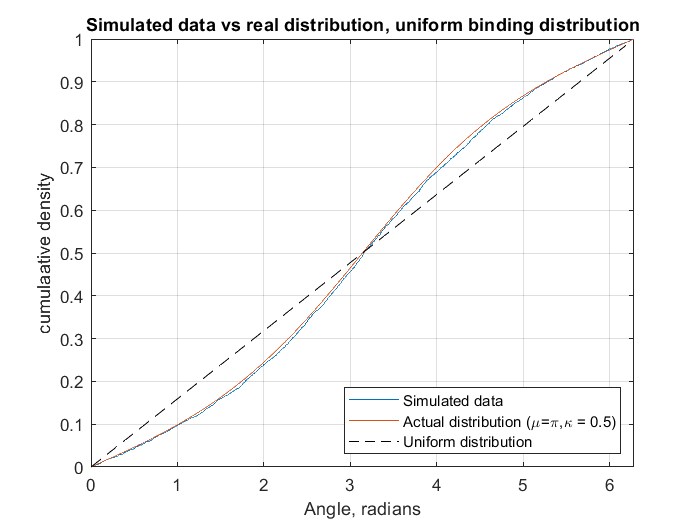
\includegraphics[width=65mm]{New Folder/MH vs real uniform binding.png}
}
\subfloat[Von Mises binding, $\kappa = \frac{1}{2}$]{
  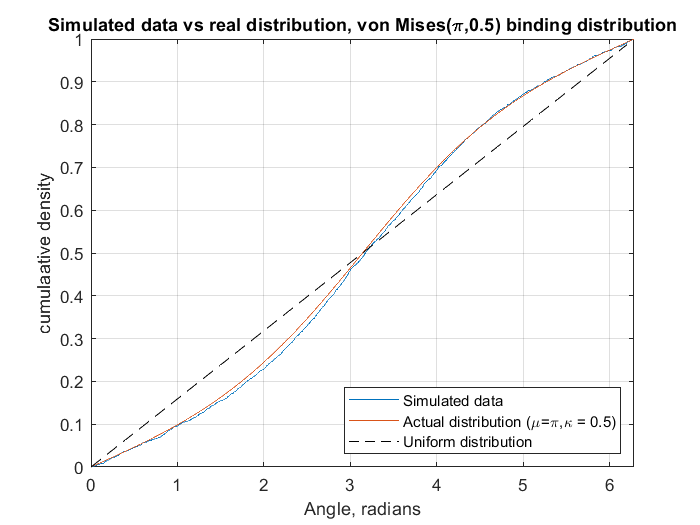
\includegraphics[width=65mm]{New Folder/MH vs real vm binding.png}
}
\newline
\subfloat[Uniform binding, $\kappa = 2$]{
  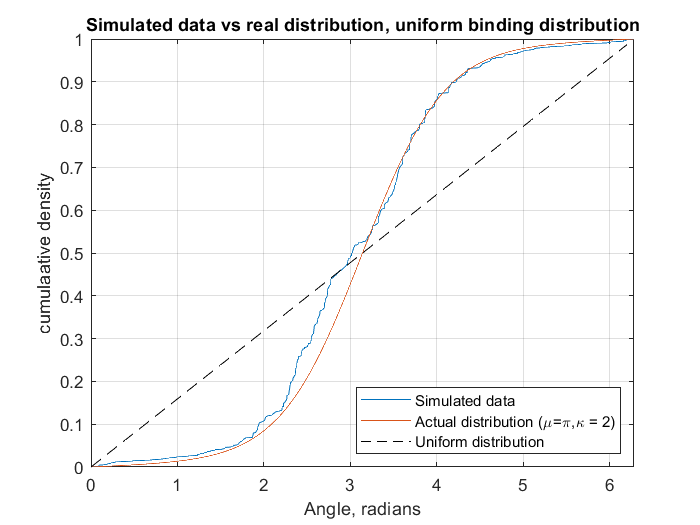
\includegraphics[width=65mm]{New Folder/MH vs real uniform 2 binding.png}
}
\subfloat[Von Mises binding, $\kappa = 2$]{
  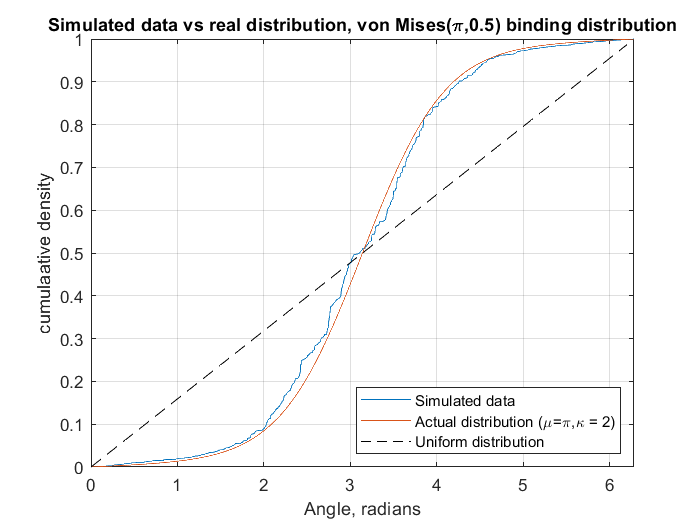
\includegraphics[width=65mm]{New Folder/MH vs real vm 2 binding.png}
}
\caption{Simulated data vs target distribution for various distributions and binding densities, $n=4000$}\label{fig:mhexamples}
\end{figure}

Then, set $\theta_{t+1}=y$ with probability $\alpha$ and $\theta_{t+1}=\theta_t$ with probability $1-\alpha$, and step forward. The expression in $\alpha$ can be thought of as a sort of likelihood function, where values of $y$ that are more "likely" to have come from $f(\theta)$ than $\theta_t$ get accepted automatically and others only get accepted with some probability $\alpha <1$ depending on their similarity to the expected distribution. Results for $\theta \in M(\mu = \pi, \kappa = \{\frac{1}{2}, 2\})$ with $n=4000$ and both a uniform and $M(\pi,\frac{1}{2})$ binding density are shown in figure \ref{fig:mhexamples}. Based purely on these results it appears that for larger values of $\kappa$ the distribution of $\{\Theta_t\}$ converges to the target distribution more slowly. 

This is a nice result, however in order to simulate realistic data our model must also have realistic autocorrelation. As we can see in figure \ref{fig:mh ac}, the simulated data has almost no autocorrelation, but data from NDBC buoys is highly autocorrelated, as we have seen for example in figure \ref{fig:ex ac}. In spite of what appears to be quick convergence to the stationary distribution, this lack of autocorrelation means that we cannot use this to generate time series of realistic data.

\begin{figure}[h]
\centering
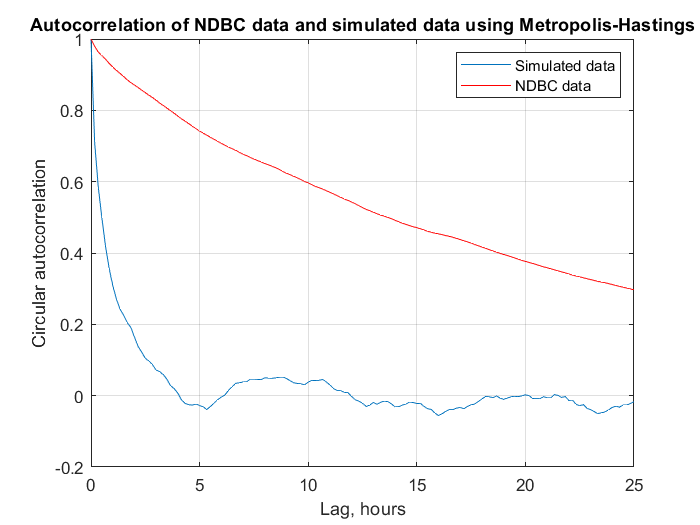
\includegraphics[width=85mm]{New Folder/ac data v model.png}
\caption{Autocorrelation of data generating using Metropolis-Hastings vs real data}\label{fig:mh ac}
\end{figure}

%\subsection{Time Series Analysis on the Circle}
%
%\subsubsection{Periodograms of circular data}
%
%Since we will want to detect periodic behavior in the time series, we will use the formulation for the periodogram of circular data given in \cite{Craig}, which is an estimate of the spectrum of a zero-mean stochastic process with length $n$. The periodogram of the zero mean process $\{x_k\}$ is given by 
%
%\begin{equation}\label{eq:pgram}
%\hat{g}(p) = \frac{1}{n}\left |{ \sum_{k=1}^n x_j \exp(i 2 \pi p k/n ) }\right | ^2
%\end{equation}
% We can detect periodicity by the relative size of $\hat{g}$. When $\hat{g}(p)$ is large there is more energy contained in the component of the process with normalized frequency $p/n$, and when it is small there is less energy. If ${x_k}$ is sampled with sampling frequency $f_s$, the real frequencies are given by $f = \frac{p}{n}f_s$. 
%
%Since any sequence of angles can be considered as a sequence of points along the unit circle, we can easily extend this formulation to circular data. Given a sequence of angles $\{x_k\} \in \left [0,2\pi \right)$ the stochastic process $\{z_k = \exp(i x_k)\}$ lies on the unit circle, and we can readily calculate its sample mean $\mu$ using equation \ref{eq:RandT}. Armed with this knowledge, it is readily seen that the periodogram of circular data is given by 
%
%\begin{equation}\label{eq:cpgram}
%\hat{g}(p) = \frac{1}{n}\left |{ \sum_{k=1}^n (z_j-\mu) \exp(i 2 \pi p k/n ) }\right | ^2
%\end{equation}
%
%Sample periodograms of both data and the model will be included in the results section to show that the temporal fluctuations follow similar patterns. We will also leverage the sample autocorrelation function, which is the subject of the next section. 

\subsection{The von Mises Process }

There are a variety of autoregressive models for data on the circle of varying complexity (see \cite{Coles}, \cite{fisher}, \cite{Harvey}, or \cite{Kato} among others, for an overview of many commonly used ones), however we will use a model based off the well-understood Ornstein-Uhlenback process \cite{oksendal}. The Ornstein-Uhlenbeck process is the solution to the stochastic differential equation

\begin{equation}\label{eq:ornuhl}
d X_t = b(t, X_t)dt+\sigma(t,X_t)dW_t
\end{equation}
where $dW_t$ is a Wiener process, that is, a continuous time stochastic process with independent, normally distributed increments with mean $0$ and variance equal to the time step so that $W_{t+\Delta t}-W_t \in N(0,\Delta t)$. This process is a modification of the continuous random walk, and can be thought of as a continuous analogue to the AR(1) process \cite{oksendal}.

One of the first continuous time processes on the circle was proposed in \cite{Kent1}. This process, known as the von Mises process, can be thought of as a continuous time analogue to the Ornstein-Uhlenbeck process \cite{Garcia}. It was defined as the solution to the familiar looking stochastic differential equation

\begin{equation}\label{eq:vmp}
d \Theta_t = \alpha \sin(\mu - \Theta_t)dt+\sigma dW_t
\end{equation}
where again $W_t$ is a Wiener process, $\alpha>0$ is a drift coefficient, $\mu$ is the mean direction, and $\sigma$ is a diffusion coefficient. This process has a unique stationary distribution given by the $M(\mu, \frac{2\alpha}{\sigma^2})$ distribution. By assuming unit time steps, this can be easily reformulated into a stochastic difference equation as

\begin{equation}\label{eq:sdiff}
\theta_{t+1} - \theta_t = \alpha \sin( \mu - \theta_t )+\sigma \epsilon_t
\end{equation}
where $\epsilon \in N(0,1)$. If we know our stationary distribution, we can develop a model using equation \ref{eq:sdiff} to generate autocorrelated data with the desired distribution. This formulation also allows us to leverage regression techniques to determine the value of $\alpha$ appropriate to match our data. 

An example of the data generated by this model is shown in figure \ref{fig:sdfig}. The data shown consists of 50000 samples generated with a target stationary distribution given by the $M(\pi/4, 2)$ distribution and with $\alpha = 0.01$. The data is strongly autocorrelated with a $1/e$ decorrelation time of approximately 15 hours assuming a sample rate of 6 samples per hour (which aligns with the NDBC data as seen in figure \ref{fig:ex ac}). Due to its inherent and tractable autocorrelation, this will be our model of choice through the remainder of the paper. 

\begin{figure}[h]
\centering
\subfloat[Sample autocorrelation of data generated from a von Mises process]{
  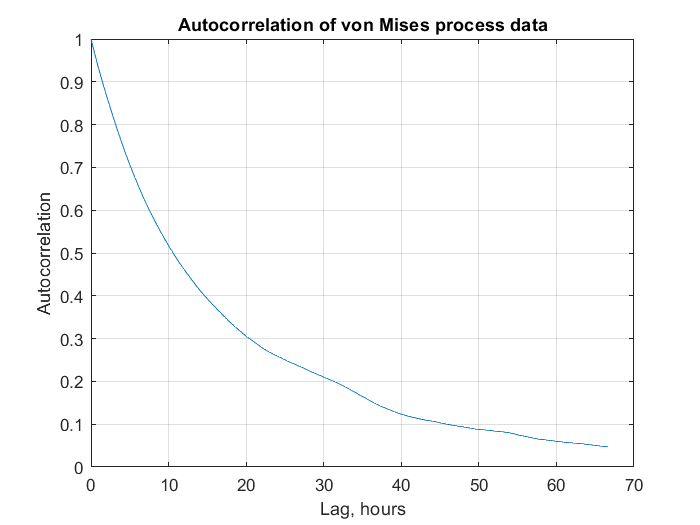
\includegraphics[width=65mm]{New Folder/ac from vm process.png}
}
\subfloat[Simulated data vs stationary distribution]{
  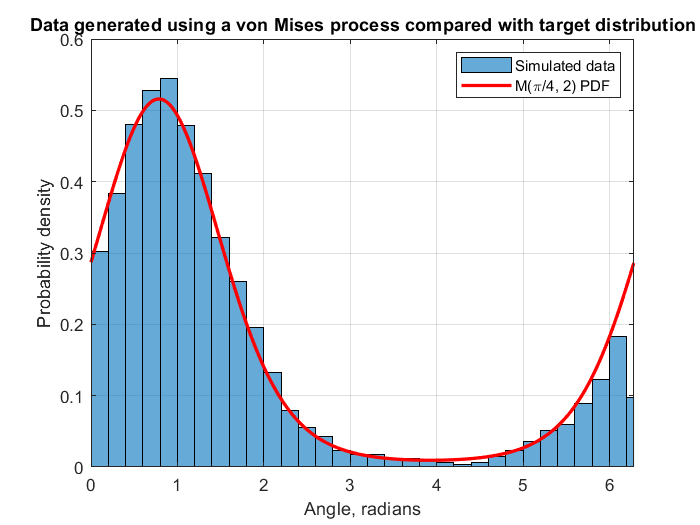
\includegraphics[width=65mm]{New Folder/vm process pdfs.png}}
\caption{Autocorrelation of simulated data and comparison with stationary distribution}\label{fig:sdfig}
\end{figure}

\section{Results}

Using the material covered thus far, a MATLAB model was developed based on equation \ref{eq:sdiff} to generate realistic time series of wind directions based on the NDBC data. The code was written specifically for this, however there are several software pacakges meant for handling circular data that could have been leveraged. One commonly used toolbox is the MATLAB CircStat toolbox described in \cite{circstat}. 

Our first task is determining appropriate values of the parameter $\alpha$ in equation \ref{eq:sdiff}. Our first attempt to match this parameter will leverage linear regression. By setting $\Delta \theta_t = \theta_{t+1} - \theta_t$ we can write equation \ref{eq:sdiff} in a format amenable to linear regression as 

\begin{equation}\label{eq:regression}
\vec{\Delta \theta} = \begin{bmatrix} \Delta \theta_1 \\ \vdots \\ \Delta \theta_{n-1} \end{bmatrix}= 
\begin{bmatrix} 1 & \sin(\mu-\theta_1) \\ \vdots & \vdots \\  1 & \sin(\mu-\theta_{n-1})  \end{bmatrix}
\begin{bmatrix} c \\ \alpha \end{bmatrix}+
\begin{bmatrix}\sigma \epsilon_1 \\ \vdots \\ \sigma \epsilon_{n-1} \end{bmatrix}
= \beta \vec{x}+\sigma \vec{\epsilon}
\end{equation}


Assuming that the noise term is relatively small, we can write an expression for $\alpha$ as

\begin{equation}\label{eq:linreg}
\begin{bmatrix} c \\ \alpha \end{bmatrix} = (\beta^T \beta)^{-1}\beta^T \vec{\Delta \theta}
\end{equation}
Due to the structure of equation \ref{eq:sdiff}, we expect that $c$ ought to be nearly zero. However, results from this method are mixed. As seen in figure \ref{fig:linreg ac}, agreement between the data and model autocorrelation functions is mixed. While in some cases, as for month 4, the autocorrelation spectra are well-matched for moderate time lags, for others such as month 1 they are not even nearly similar past very short lags\footnote{We do not care about matching long-time (i.e. $\ge$ 30 hours) autocorrelation since the data is not meaningfully correlated that far out, but we do care for short times where data is highly autocorrelated}. 

\begin{figure}[h]
\centering
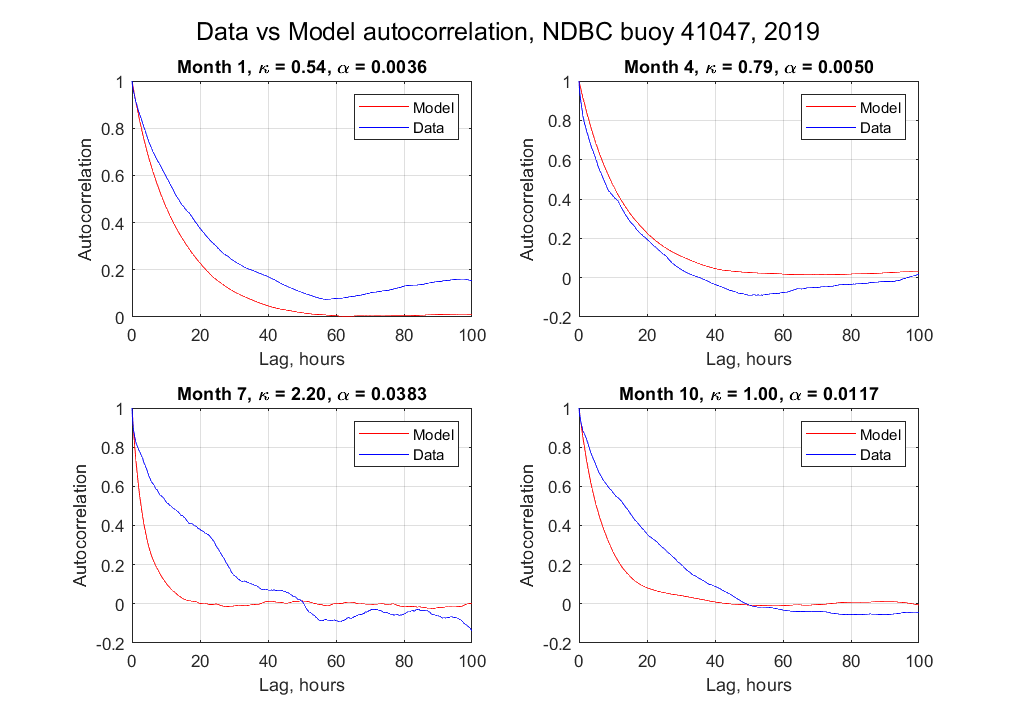
\includegraphics[width=100mm]{New Folder/data v model autocorrelation.png}
\caption{Model vs data autocorrelation with $\alpha$ calculated by linear regression}\label{fig:linreg ac}
\end{figure}

However, as we can recall from the discussion in section \ref{correlation} and see in figures \ref{fig:ex ac} and \ref{fig:linreg ac}, the autocorrelation is, at least where $\hat{\rho}\ge 0.2$, very nearly an exponential decay. With this in mind, we can suggest a different way to determine an appropriate value of $\alpha$ by matching the $1/e$ decorrelation time. If we want the data to be exponentially autocorrelated with a $1/e$ decorrelation time of $n$ samples, we can set $\alpha = \frac{1}{n}$, and then we will have an autocorrelation function $\rho(m) = e^{-\frac{m}{n}}$, where $m$ is in samples. By setting $n$ to the $1/e$ decorrelation of the data in samples and setting $\alpha$ accordingly, we generate the results shown in figure \ref{fig:match decorr ac}. We can see that the results match the data better in month 7 and month 10, however the performance is worse for months 1 and 4. In this method, it appears that we are better able to match the autocorrelation for high values of $\kappa$ than lower values. 

\begin{figure}[h]
\centering
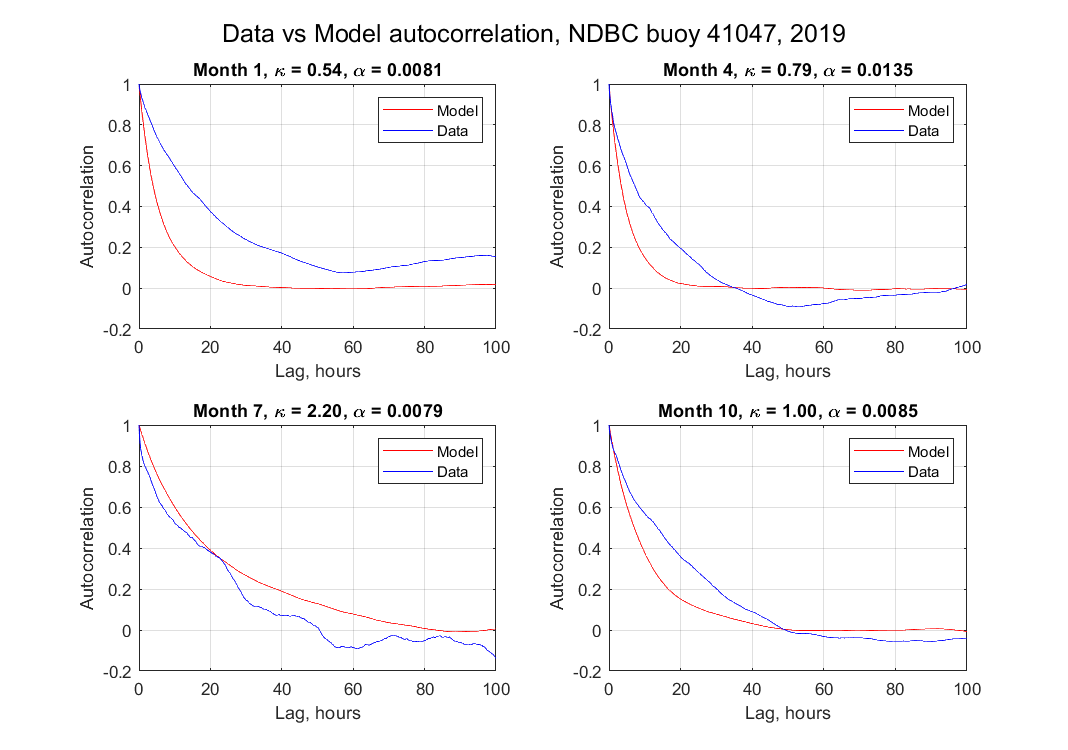
\includegraphics[width=100mm]{New Folder/data v model autocorrelation match decorr time.png}
\caption{Model vs data autocorrelation with $\alpha$ calculated by matching decorrelation time}\label{fig:match decorr ac}
\end{figure}

We can see this trend continue with data from buoy 41010 taken in 2018, where the months with higher values of $\kappa$ have a modeled autocorrelation that seems to provide a decent fit to the data autocorrelation. Generally, this method performs best when $\kappa >  1$. 

\begin{figure}[h]
\centering
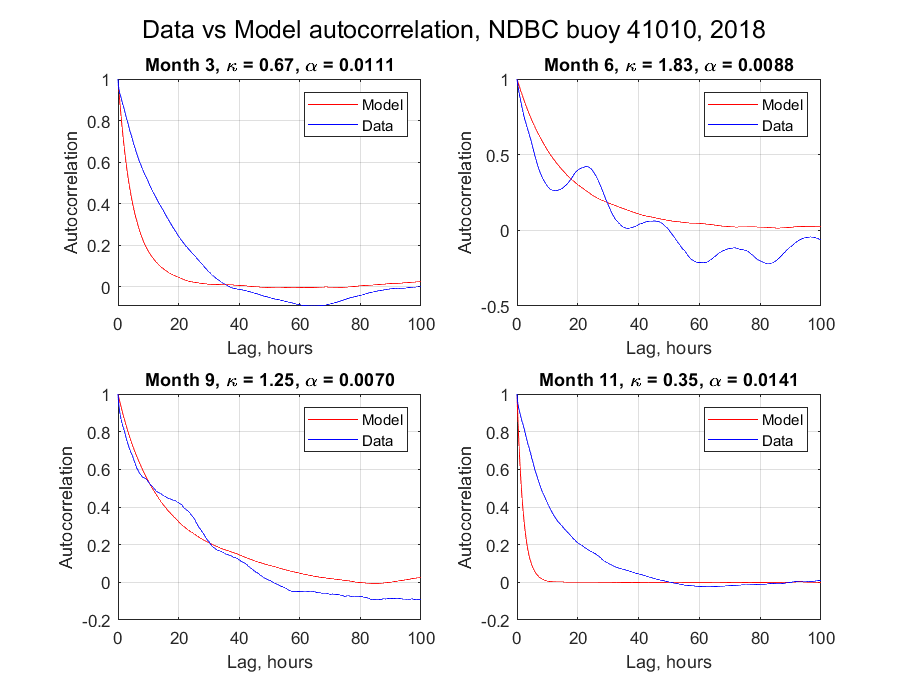
\includegraphics[width=100mm]{New Folder/data v model ac 41010 2018 match decorr.png}
\caption{Buoy 41010, autocorrelation generated by matching decorrelation time}\label{fig:linreg ac}
\end{figure}

With this in mind, we want to determine what the actual effect of $\kappa$ on the error in decorrelation time might be for both of our methods of calculating $\alpha$: by matching decorrelation time and by performing linear regression. To do the calculation, every usable month of data available was processed, and a maximum likelihood estimate of $\kappa$ was calculated. Then the value of $\alpha$ was estimated by linear regression and by matching decorrelation time, and the difference between the decorrelation time shown by the data and the model in hours was recorded. By doing this, we see hard evidence for what was postulated in the previous paragraph: As the value of $\kappa$ increases, we are better able to match the decorrelation time seen in the data when we set $\alpha$ to match it, but when we use linear regression to find $\alpha$ we are less able to properly match the decorrelation time. By shoosing $\alpha$, we are able to match decorrelation time to within about 5 hours for $\kappa \ge 1.5$ and nearly within 10 hours for $\kappa \ge 1$, which, while far from perfect, is notably better than the results when $\alpha$ is calculated via linear regression.

This is not entirely unexpected, since if we expect equation $\ref{eq:sdiff}$ to be a good match for the data we can see that the variance of the noise term $\sigma^2$ is related to $\alpha$ by the relation $\kappa =\frac{2\alpha}{\sigma^2}$, so $\sigma^2 = \frac{2\alpha}{\kappa}$ and the noise term is similar in size to the magnitude of the $\alpha \sin(\mu-\theta_t)$ term or even much larger than it, which makes linear regression difficult. And when $\kappa$ is large, the data is more concentrated around $\mu$ so $\alpha \sin(\mu-\theta_t) \approx \alpha (\mu-\theta_t)$ more often, so our von Mises process is more like an $AR(1)$ process and the autocorrelation is closer to an exponential decay, which we assumed to calculate $\alpha$ in the first place.

\begin{figure}[h]
\centering
\subfloat[$\alpha$ chosen to match decorrelation]{
  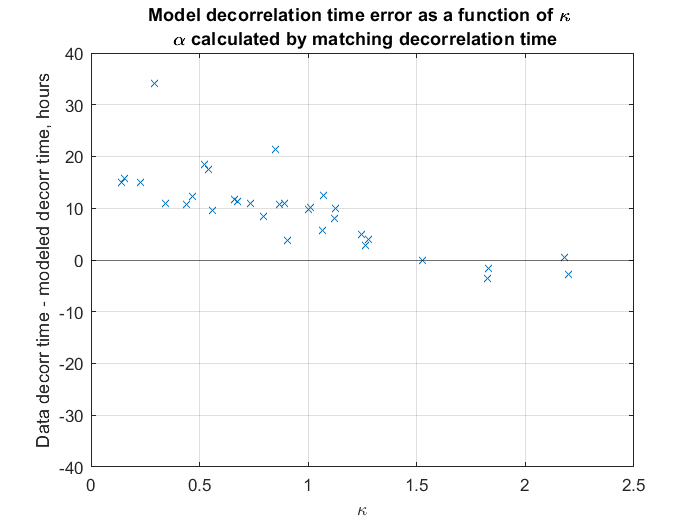
\includegraphics[width=65mm]{New Folder/decorr error vs kappa.png}
}
\subfloat[$\alpha$ chosen by linear regression]{
  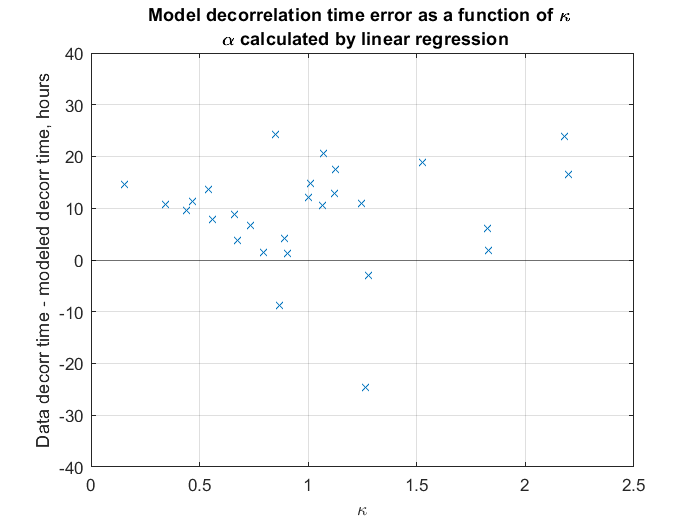
\includegraphics[width=65mm]{New Folder/decorr error vs kappa lin reg.png}}
\caption{The effect of $\kappa$ on matching autocorrelation for both methods of estimating $\alpha$}\label{fig:matching decorr}
\end{figure}

Lastly, we want to be able to demonstrate that we generate data that matches the assumed distributions. While we have seen an example of this in figure \ref{fig:sdfig} for a large number of datapoints, we want to get an idea of how quickly we converge to the assumed distribution. noting that there are only about 4000 samples of wind direction taken in each month, we would like to be able to converge to the stationary distribution without exceeding that value too much. To investigate convergence, several sequences of $10^6$ datapoints were generated with $\mu=0$ and values of $\kappa$ ranging from $0.5$ to $4$ to cover the approximate range of values of $\kappa$ seen in the data. Maximum likelihood estimates of $\mu$ and $\kappa$ were calculated for the first $n$ samples, for $10^3 \le n \le 10^6$. Error in $\mu$ is measured by equation \ref{eq:cosdist} and error in $\kappa$ is measured by percent error. From this, we can see that while the model converges to the mean of the stationary distribution quickly, it takes much longer to get an estimate of $\kappa$ that is within $10 \%$ of the stationary value, in this case requiring well over $10^4$ samples. More importantly, for ~$4000$ samples, the error in the estimate of $\kappa$ can be more than $20 \%$. The convergence is much slower than for the data generated using the Metropolis-Hastings method, which generated data matching the target distribution within the desired ~$4000$ points. 

\begin{figure}[h]
\centering
\subfloat[Angular error in the estimate of $\mu$ vs $n$]{
  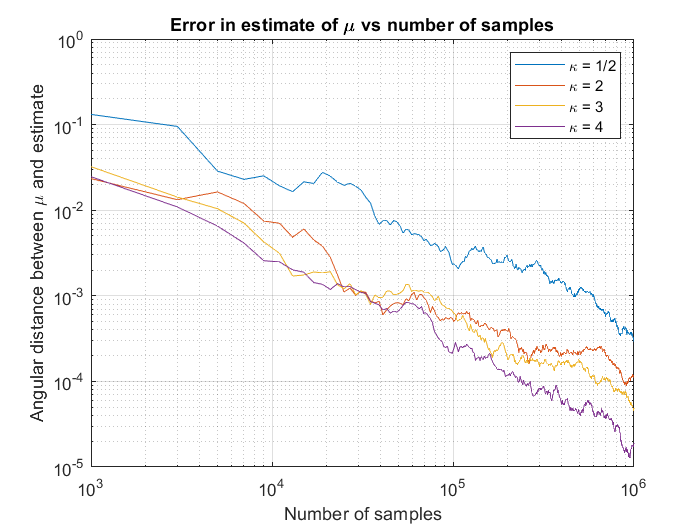
\includegraphics[width=65mm]{New Folder/mu error final.png}
}
\subfloat[Percent error in the estimate of $\kappa$ vs $n$]{
  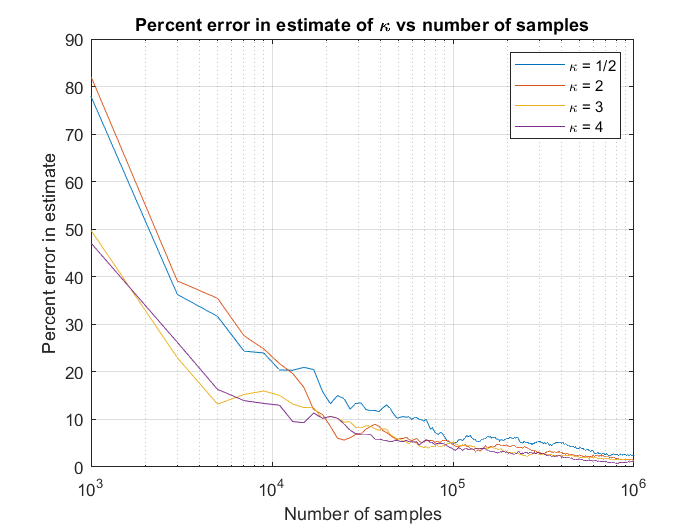
\includegraphics[width=65mm]{New Folder/kappa error final.png}}
\caption{Error in the estimates of $\mu$ and $\kappa$ for varying $\kappa$}\label{fig:convergence}
\end{figure}

Whether this is an acceptable level of error or not depends on how exact you wish your modeling to be. In our case, this slow convergence to the stationary distribution means that unless we are generating large amounts of data we cannot guarantee that the data approximates the stationary distribution well. This can be readily seen by plotting the empircal CDFs of the NDBC data and the same number of simulated data points on the same axes. While sometimes we are able to get data that has a reasonably similar distribution to the NDBC data, we are just as often unable to do so, as seen in figure \ref{fig:match to data}. Sometimes we get close to the assumed stationary distribution (shown in black) as when mimicking the buoy 41047 data from October 2019 (or, at least, we are no further away than the data is), and sometimes we are not remotely close, as seen when we try to simulate the data from buoy 41010 in December 2018. 

\begin{figure}[h]
\centering
\subfloat[Buoy 41047, Oct 2019]{
  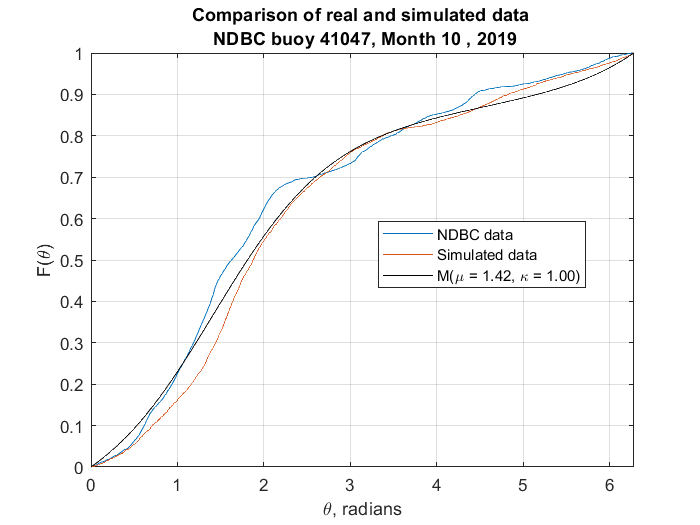
\includegraphics[width=65mm]{New Folder/sim vs data 41047 10 2019.png}
}
\subfloat[Buoy 41010, Dec 2018]{
  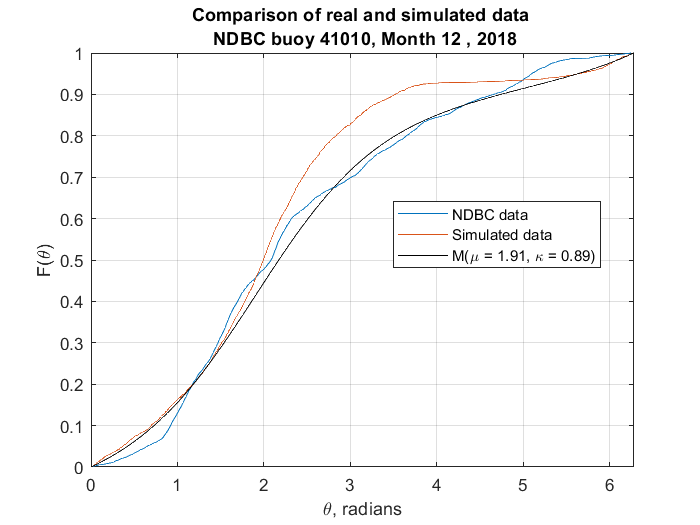
\includegraphics[width=65mm]{New Folder/sim vs data 41010 12 2018.png}}
\caption{Comparison between simulated and real NDBC data}\label{fig:match to data}
\end{figure}

So, while the model is able to generate autocorrelated data with a von Mises distribution, the data does not match the spread of the stationary distribution of the von Mises process well without generating a large amount of data points and the autocorrelation is difficult to get exactly right. There is one more feature of the data thar the model does not properly capture. When the data is unwrapped, it appears to have a strong drift term. This suggests that the wind direction is varying in a periodic way, and while it may be concentrated in a certain direction some sort of geophysical process causes it to move around the circle in a fairly periodic way. However, we do not see that in the simulated data because there is no drift term like there appears to be in some cases in the data. This geophysical process is likely also driving the autocorrelation we see in the data. One possible extension of this model to better match the data could involve a drift term on the unwrapped angular data. 

\begin{figure}[h]
\centering
\subfloat[Simulated data]{
  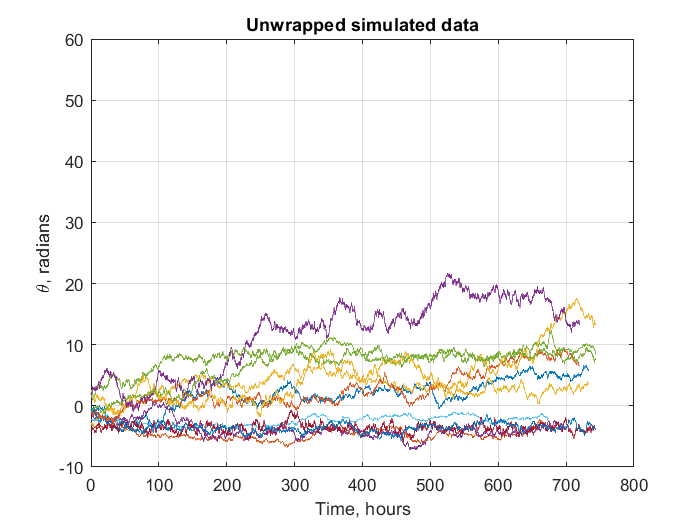
\includegraphics[width=65mm]{New Folder/unwrapped sim data.png}
}
\subfloat[Real data]{
  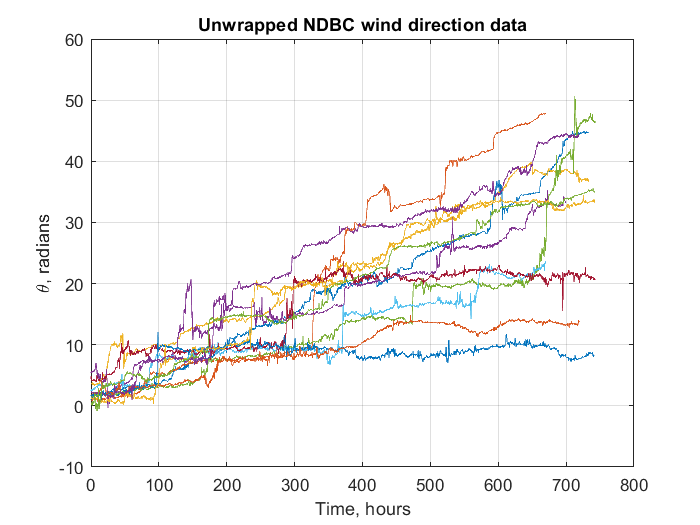
\includegraphics[width=65mm]{New Folder/unwrapped wind direction data.png}}
\caption{Unwrapped simulated and real data}\label{fig:unwrap}
\end{figure}

\section{Conclusions}

We introduced the concept of directional or circular statistics and two commonly used distributions on the circle, and analyzed two simple methods of generating data with a von Mises distribution. We showed that the von Mises process shown in equation \ref{eq:vmp} can be used to generate an autocorrelated time series of angular data that has a stationary von Mises distribution, and we compared results from simulations using that process to wind direction data collected by the National Data Buoy Center in the Atlantic Ocean. While the model was able to capture the autocorrelation of the data and would, given enough time, match the distribution of the deat as well, it required a large number of samples to accurately model the staionary distribution and did not match other properties of the data properly. We suggest that, while this model performs reasonably well given that it is exceedingly simple, it is likely more appropriate to simulate this sort of data using higher order models such as one of the many flavors of ARMA(p,q) models suggested in, for example, \cite{Harvey}, among others. Several other such models are listed in the bibliography. 

\begin{thebibliography}{1}

\bibitem{Al Yammahi} Al Yammahi, Aishah \& Prashanth R. Marpu \& Taha B. M. J. Ouarda (2021), ''Modeling directional distributions of wind data in the United
Arab Emirates at different elevations'', Arabian Journal of Geosciences

\bibitem{Rinaldo} Artes, Rinaldo \& Clelia M. C. Toloi (2009) An Autoregressive Model for Time
Series of Circular Data, Communications in Statistics - Theory and Methods, 39:1, 186-194, DOI:
10.1080/03610920802650338

\bibitem{circstat} Berens, Phillipp (2009) CircStat: A MATLAB Toolbox for Circular Statistics. Journal of Statistical Software Volume 31 Issue 10

\bibitem{borradaile} Borradaile, G. J. (2003). Statistics of earth science data : their distribution in time, space, and orientation. Springer. ISBN 978-3-662-05223-5

\bibitem{Broemling} Broemeling, Lyle D. (1 November 2011). "An Account of Early Statistical Inference in Arab Cryptology". The American Statistician. 65 (4): 255–257. doi:10.1198/tas.2011.10191

\bibitem{Coles} Coles, S. G. (1998). Inference for circular distributions and processes. Statistical Computing, 5

\bibitem{Craig} Craig, Peter S (1988), ''Time Series Analysis for Directional Data'', Phd Thesis

\bibitem{fisher} Fisher, N.I and A.J. Lee (1994), ''Time Series Analysis of Circular Data'', Journal of the Royal Statistical Society. Series B

\bibitem{Garcia}  García-Portugués, Eduardo, Michael Sørensen, Kanti V. Mardia, and Thomas Hamelryck (2019), "Langevin diffusions on the torus: estimation and applications", Statistics and Computing

\bibitem{Gubner}Gubner, John A. (2006). Probability and Random Processes for Electrical and Computer Engineers. Cambridge University Press. ISBN 978-0-521-86470-1

\bibitem{Harvey} Harvey, Andrew; Hurn,Stan, and Stephen Thiele (2019) "Modeling Directional (Circular) Time Series", https://doi.org/10.17863/CAM.43915

\bibitem{Holzmann} Holzmann H, Munk A, Suster M, Zucchini W (2006) Hidden Markov models for circular and linear–circular
time series. Environ Ecol Stat 13:325–347

\bibitem{Johnson} Johnson RA, Wehrly TE (1979) Bivariate models for dependence of angular observations and a
related Markov process. Biometrika 66:255–2566

\bibitem{Kato} Kato,Shogo (2010); "A Markov Process for Circular Data" , Journal of the Royal Statistical Society. Series B (Statistical Methodology)

\bibitem{Kent1} Kent, J. (1975). Discussion of paper by K. V. Mardia. J. Roy. Statist. Soc. Ser. B, 37(3):377–378

\bibitem{Kuiper} Kuiper, N. H. (1960) "Tests concerning random points on a circle". Proceedings of the Koninklijke Nederlandse Akademie van Wetenschappen, Series A. 63: 38–47.

\bibitem{Larsen}Larsen, Richard J and Morris L. Marx, ''An Introduction to Mathematical Statistics and Its Applications, 6th Edition'', Pearson Education, 2018

\bibitem{Mahrt} Mahrt, Larry (2011) ''Surface Wind Direction Variability'',  Journal of Applied Meteorology and Climatology, 

\bibitem{Kanti}Mardia, Kantil; Jupp, Peter E. (1999). Directional Statistics. Wiley. ISBN 978-0-471-95333-3.

\bibitem{Mardia2} Mardia, K. V. (1975), "Statistics of Directional Data", Read before the Royal Statistical Society at a meeting organized by the Research Section on Wednesday, March 19th, 1975

\bibitem{Metropolis}Metropolis, N., A.  Rosenbluth, M.  Rosenbluth, A.  Teller, and E. Teller (1953), Equation of state calculation by fast computing machines, J. Chem. Phys., 21, 1087-1092

\bibitem{NDBC} National Data Buoy Center, https://www.ndbc.noaa.gov/

\bibitem{oksendal} Øksendal, Bernt (2007), Stochastic Differential Equations: An Introduction with Applications, Sixth Edition, Springer-Verlag Heidelberg New York

\bibitem{NDBCdoc} Programmatic Environmental Assessment For the National Oceanic and Atmospheric Administration National Data Buoy Center (2018)  
\end{thebibliography}

\appendix
\section{Project git repository}
The code and references used for this project (along with other papers that were not referenced but that the reader may find interesting) are located in a github repository at HYPERLINK. To run the code, first run the script startAnalysis.m. The model is run in analysis/sdemodel.m. Other scripts in the analysis folder are mostly from starting or stopping down a certain path during modeling. Documentation is incomplete but at this point the code as written generally assumes angles are in radians. 

 The MATLAB code for the CircStat toolbox can be found on the MATLAB file exchange at https://www.mathworks.com/matlabcentral/fileexchange/10676-circular-statistics-toolbox-directional-statistics.

\end{document}